% 8-minute talk on "Can Power Draw Constrain Covert Compute?" (paper/main.tex).
% for 16x9 (modern wide screen) aspect ratio slides
\documentclass[aspectratio=169]{beamer}

% Oxford Maths theming
\usetheme{oxfordmaths}
\usepackage{xcolor}

% Drop the infolines headline (section/subsection name above each frame title)
\setbeamertemplate{headline}{}

% ===== Semantic color palette (matched to the paper's figures) =====
% Declared / honest work
\colorlet{colDec}{teal!60!black}
% Covert work / the adversary
\colorlet{colCov}{orange!85!black}
% The power trace / the meter
\colorlet{colTrace}{blue!55!black}
% Warnings / the punchline
\colorlet{colWarnLine}{red!70!black}

\hypersetup{colorlinks=true, urlcolor=teal, linkcolor=., filecolor=.}
% MATS logo is placed by a tikz overlay on the title frame (below), not via
% \titlelogo: the theme hook pins it small in the bottom-right corner.

% Set author etc info
\title[Power $\to$ FLOPs]{Can Power Draw Constrain Covert Compute?}
\author[Tom Kimpson]{Tom Kimpson}
\institute{University of Melbourne \& MATS\\[4pt]
	{\small with Mauricio Baker, Emlyn Graham, Anjay Friedman,
	Maximus Rafla, Coby Joseph}}
% PLACEHOLDER date/venue -- update before the talk.
\date[2026]{MATS, August 2026}

% ===== Packages & helpers =====
\usepackage{amsmath, amssymb, mathtools}
\usepackage{booktabs}
\usepackage{tikz}
\usetikzlibrary{arrows.meta, positioning, calc, decorations.pathreplacing, fit}
\usepackage{graphicx}
% All included PDFs are the paper's regenerable figures.
\graphicspath{{../figures/}}

% Reduce cluttered bullets
\setbeamertemplate{itemize items}[circle]
\setbeamertemplate{enumerate items}[default]

% Backup slide commands to exclude appendix from total count
\newcommand{\backupbegin}{
	\newcounter{framenumberappendix}
	\setcounter{framenumberappendix}{\value{framenumber}}
}
\newcommand{\backupend}{
	\setcounter{framenumber}{\value{framenumberappendix}}
}

% Page number template
\makeatletter
\setbeamertemplate{page number in head/foot}{%
	\insertframenumber
}
\makeatother


\begin{document}

% ===== Title =====
\begin{frame}[plain]
	\titlepage
	\begin{tikzpicture}[remember picture, overlay]
		\node[anchor=north east, inner sep=0pt]
			at ([xshift=-7mm, yshift=-6mm]current page.north east)
			{
\includegraphics[width=\dimexpr\paperwidth/4\relax]{figures/mats_red_acronym.png}};
	\end{tikzpicture}
\end{frame}


% ================================================================
% SLIDE 2: Why verify compute? (+ the two-questions nod)
% ================================================================
\begin{frame}{Why Verify Compute?}
	\small
	\begin{itemize}\itemsep4pt
		\item AI governance agreements require \textbf{verification}.
		\item An outside party (``verifier'') must be able to check what a
		compute operator (``prover'') \emph{actually ran}.
	\end{itemize}

	\vspace{3mm}
	\centering
	% The prover--verifier game at its most general: a declaration plus
	% supporting evidence, and the two checks the verifier owes. Power is
	% deliberately absent; the meter enters on the next slide.
	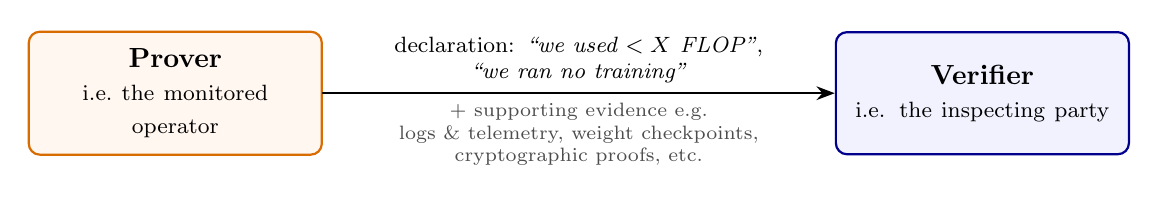
\begin{tikzpicture}[>=Stealth, line cap=round,
		party/.style={draw, thick, rounded corners=4pt, align=center,
			inner sep=6pt, text width=3.3cm, minimum height=1.55cm}]

		\node[party, draw=colCov, fill=orange!6] (prover) at (0,0)
			{\textbf{Prover}\\
			{\footnotesize i.e.\ the \mbox{monitored} operator}};

		\node[party, draw=colTrace, fill=blue!5] (verifier) at (10.25,0)
			{\textbf{Verifier}\\
			{\footnotesize i.e. the inspecting party}};

		% a declaration, plus the "stuff" that lets the verifier check it
		\draw[->, thick] (prover.east) -- (verifier.west)
			node[midway, above, font=\footnotesize, align=center]
				{declaration: \emph{``we used $< X$ FLOP''},\\
				\emph{``we ran no training''}}
			node[midway, below, font=\scriptsize, text=gray!60!black,
				align=center]
				{+ supporting evidence e.g. \\
				logs \& telemetry, weight checkpoints,\\
				cryptographic proofs, etc.};
	\end{tikzpicture}
\end{frame}




% ================================================================
% SLIDE 2: the adversary, and why off-chip sensing (+ the nod)
% ================================================================
\begin{frame}{Verification Must Survive an Adversary}
	\small
	\begin{itemize}\itemsep4pt
		\item The prover may \textbf{not behave honestly} --- try to hide compute, try to run training 
		\item ``Evidence" is provided by the (cheating?) prover based on \emph{silicon the
		prover controls}, e.g. utilisation counters, on-chip clocks, attested firmware, etc.
		\item \textbf{Off-chip analogue sensors} (power, EM, acoustic, thermal)
		bypass that: physically separate, retrofittable, securable against
		tampering.
	\end{itemize}
\end{frame}


% ================================================================
% SLIDE 4: this work --- the power channel, and the two questions
% ================================================================
\begin{frame}{This Work:  Power Channel}
	\small
	We focus on one analogue channel: \textbf{power draw} ---  \emph{every operation costs energy}.
	\par\normalsize

	\vspace{2mm}
	\centering
	% The slide-2 game again, now with the second channel drawn in: the
	% off-chip meter hands the verifier something to check the claim against.
	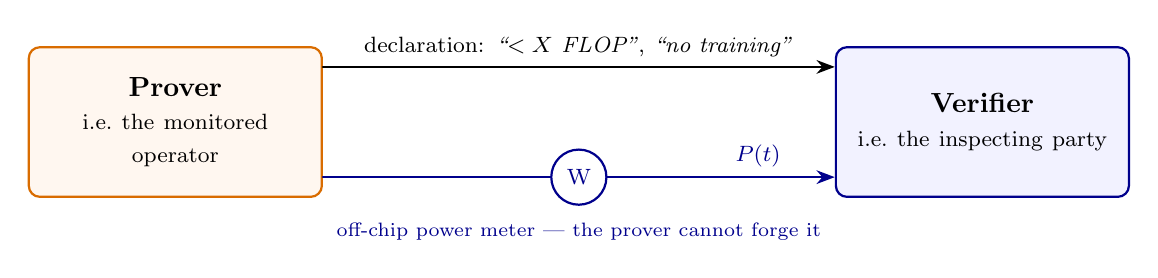
\begin{tikzpicture}[>=Stealth, line cap=round,
		party/.style={draw, thick, rounded corners=4pt, align=center,
			inner sep=6pt, text width=3.3cm, minimum height=1.9cm}]

		\node[party, draw=colCov, fill=orange!6] (prover) at (0,0)
			{\textbf{Prover}\\
			{\footnotesize i.e.\ the \mbox{monitored} operator}};

		\node[party, draw=colTrace, fill=blue!5] (verifier) at (10.25,0)
			{\textbf{Verifier}\\
			{\footnotesize i.e.\ the inspecting party}};

		% channel 1: the declaration (a claim)
		\draw[->, thick] ([yshift=7mm]prover.east) -- ([yshift=7mm]verifier.west)
			node[midway, above, font=\footnotesize]
				{declaration: \emph{``$< X$ FLOP''}, \emph{``no training''}};

		% channel 2: the power feed, tapped by an off-chip meter
		\draw[->, thick, colTrace]
			([yshift=-7mm]prover.east) -- ([yshift=-7mm]verifier.west)
			node[pos=0.85, above, font=\footnotesize, text=colTrace] {$P(t)$};
		\node[circle, draw=colTrace, thick, fill=white, minimum size=7mm,
			font=\footnotesize, text=colTrace] (meter)
			at ([yshift=-7mm]$(prover.east)!0.5!(verifier.west)$) {W};
		\node[font=\scriptsize, text=colTrace, anchor=north]
			at ([yshift=-1mm]meter.south)
			{off-chip power meter --- the prover cannot forge it};
	\end{tikzpicture}

	\vspace{3mm}
	% The two questions the trace can be asked of the declaration. Left box
	% is the companion paper's territory and is deliberately greyed.
	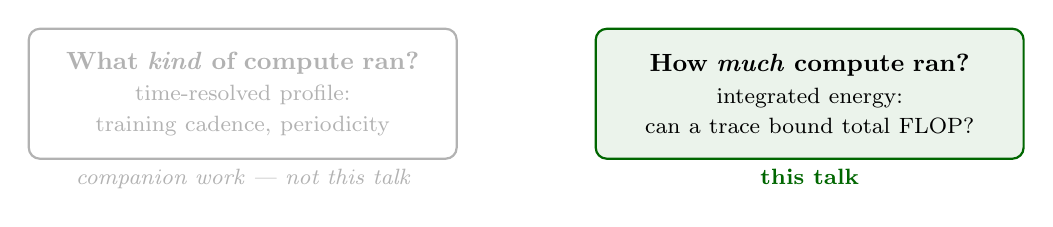
\begin{tikzpicture}[
		qbox/.style={draw, thick, rounded corners=4pt, align=center,
			minimum height=1.65cm, text width=5.2cm, font=\small},
		>=Stealth
	]
		\node[qbox, draw=gray!60, text=gray!60] (kind) at (0,0)
			{\textbf{What \emph{kind} of compute ran?}\\[2pt]
			{\footnotesize time-resolved profile:\\ training cadence, periodicity}};
		\node[qbox, draw=green!40!black, fill=green!40!black!8] (much) at (7.2,0)
			{\textbf{How \emph{much} compute ran?}\\[2pt]
			{\footnotesize integrated energy:\\ can a trace bound total FLOP?}};
		\node[font=\footnotesize\itshape, text=gray!60, anchor=north]
			at (kind.south) {companion work --- not this talk};
		\node[font=\footnotesize\bfseries, text=green!40!black, anchor=north]
			at (much.south) {this talk};
	\end{tikzpicture}
\end{frame}






% ================================================================
% SLIDE 3: The meter sees only a product (many-to-one)
% ================================================================
\begin{frame}{What The Meter Sees}
	% The forward model, with each symbol priced in words.
	\vspace{-1mm}
	\begin{equation*}
		\underbrace{P(t)}_{\substack{\text{what the}\\ \text{meter sees}}}
		\;=\;
		\underbrace{{\color{colCov} r(t)}}_{\substack{\text{pJ/op: prover's}\\ \text{choice, invisible}}}
		\;\cdot\;
		\underbrace{{\color{colDec} F(t)}}_{\substack{\text{op/s: what the}\\ \text{verifier wants}}}
		\;+\;
		\underbrace{ \color{colCov} P_0(t)}_{\substack{\text{overhead:}\\ \text{idle, cooling}}}
	\end{equation*}

	\vspace{1mm}
	\centering
	% Port of the paper's fig:noninjective: two workloads -> one trace ->
	% set-valued inversion.
	\resizebox{0.90\textwidth}{!}{%
	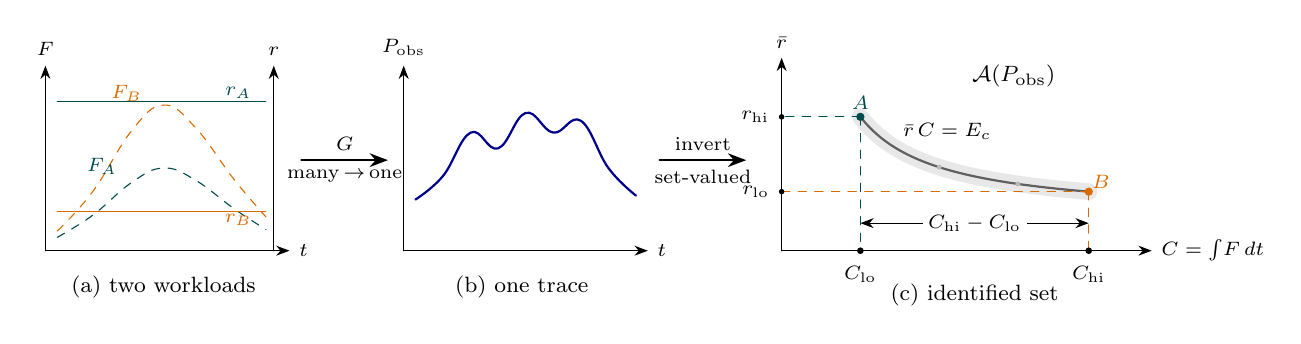
\begin{tikzpicture}[>=Stealth, line join=round, line cap=round]

		% ================= (a) two admissible workloads =================
		\begin{scope}[shift={(0,0)}]
			\draw[->] (0,0.55) -- (3.1,0.55) node[right] {\scriptsize $t$};
			\draw[->] (0,0.55) -- (0,2.9) node[above] {\scriptsize $F$};
			\draw[->] (2.9,0.55) -- (2.9,2.9) node[above] {\scriptsize $r$};
			\draw[colDec] (0.15,2.45) -- (2.8,2.45);
			\draw[colDec, dashed] plot[smooth, tension=0.7] coordinates
			{(0.15,0.72) (0.6,1.0) (1.1,1.42) (1.5,1.6) (1.9,1.45) (2.4,1.08) (2.8,0.82)};
			\draw[colCov] (0.15,1.05) -- (2.8,1.05);
			\draw[colCov, dashed] plot[smooth, tension=0.7] coordinates
			{(0.15,0.8) (0.6,1.3) (1.1,2.08) (1.5,2.4) (1.9,2.12) (2.4,1.45) (2.8,0.98)};
			\node[colDec, anchor=south, inner sep=0.5pt] at (2.45,2.46) {\scriptsize $r_A$};
			\node[colCov, anchor=north, inner sep=0.5pt] at (2.45,1.04) {\scriptsize $r_B$};
			\node[colDec, anchor=east, inner sep=1pt] at (0.95,1.62) {\scriptsize $F_A$};
			\node[colCov, anchor=south east, inner sep=0.5pt] at (1.25,2.42) {\scriptsize $F_B$};
			\node[anchor=north] at (1.5,0.35) {\footnotesize (a) two workloads};
		\end{scope}

		\draw[->, thick] (3.25,1.7) -- (4.35,1.7);
		\node[anchor=south, inner sep=1pt] at (3.8,1.78) {\scriptsize $G$};
		\node[anchor=north, inner sep=1pt] at (3.8,1.62) {\scriptsize many$\,\to\,$one};

		% ================= (b) one power trace =================
		\begin{scope}[shift={(4.55,0)}]
			\draw[->] (0,0.55) -- (3.1,0.55) node[right] {\scriptsize $t$};
			\draw[->] (0,0.55) -- (0,2.9) node[above] {\scriptsize $P_{\mathrm{obs}}$};
			\draw[thick, colTrace] plot[smooth, tension=0.7] coordinates
			{(0.15,1.2) (0.5,1.5) (0.85,2.05) (1.2,1.85) (1.55,2.3)
				(1.9,2.05) (2.25,2.2) (2.6,1.6) (2.95,1.25)};
			\node[anchor=north] at (1.5,0.35) {\footnotesize (b) one trace};
		\end{scope}

		\draw[->, thick] (7.8,1.7) -- (8.9,1.7);
		\node[anchor=south, inner sep=1pt] at (8.35,1.78) {\scriptsize invert};
		\node[anchor=north, inner sep=1pt] at (8.35,1.62) {\scriptsize set-valued};

		% ================= (c) identified set = constant-energy arc =================
		\begin{scope}[shift={(9.35,0)}]
			\draw[->] (0,0.55) -- (4.7,0.55)
				node[right] {\scriptsize $C = \int\! F\,dt$};
			\draw[->] (0,0.55) -- (0,3.0) node[above] {\scriptsize $\bar r$};
			\draw[line width=6pt, gray!18, line cap=round, smooth, samples=60, domain=1.0:3.9]
			plot (\x,{1.2776/\x+0.9724});
			\draw[gray!75!black, thick, smooth, samples=60, domain=1.0:3.9]
			plot (\x,{1.2776/\x+0.9724});
			\node[anchor=south west, inner sep=1pt] at (1.5,1.92) {\scriptsize $\bar r\,C=E_c$};
			\node[anchor=south] at (2.95,2.5) {\footnotesize $\mathcal{A}(P_{\mathrm{obs}})$};
			\fill[gray!55] (2.0,1.611) circle (0.9pt);
			\fill[gray!55] (3.0,1.398) circle (0.9pt);
			\fill[colDec]   (1.0,2.25) circle (1.5pt) node[above, inner sep=2.5pt] {\scriptsize $A$};
			\fill[colCov] (3.9,1.3)  circle (1.5pt) node[above right, inner sep=1pt] {\scriptsize $B$};
			\draw[dashed, colDec]   (1.0,2.25) -- (0,2.25);
			\draw[dashed, colCov] (3.9,1.3)  -- (0,1.3);
			\fill (0,2.25) circle (1.0pt) node[left=1pt] {\scriptsize $r_{\mathrm{hi}}$};
			\fill (0,1.3)  circle (1.0pt) node[left=1pt] {\scriptsize $r_{\mathrm{lo}}$};
			\draw[dashed, colDec]   (1.0,2.25) -- (1.0,0.55);
			\draw[dashed, colCov] (3.9,1.3)  -- (3.9,0.55);
			\fill (1.0,0.55) circle (1.2pt) node[below=2pt] {\scriptsize $C_{\mathrm{lo}}$};
			\fill (3.9,0.55) circle (1.2pt) node[below=2pt] {\scriptsize $C_{\mathrm{hi}}$};
			\draw[<->] (1.0,0.9) -- (3.9,0.9) node[midway, fill=white, inner sep=2pt] {\scriptsize $C_{\mathrm{hi}} - C_{\mathrm{lo}}$};
			\node[anchor=north] at (2.45,0.25) {\footnotesize (c) identified set};
		\end{scope}

	\end{tikzpicture}%
	}

	\vspace{1mm}
	\centering
	\alert{Goal}: bound the width $C_{\mathrm{hi}} - C_{\mathrm{lo}} = C_{\mathrm{hi}} - C_{\mathrm{dec}} = C_{\mathrm{covert}}^{\mathrm{max}}$
	%\vspace{-1mm}
	%\begin{equation*}\small
		%C_{\mathrm{hi}} - C_{\mathrm{lo}} \;\le\;
		%\frac{\bigl(r_{\mathrm{hi}}^{\mathrm{dec}} - r_{\mathrm{lo}}^{\mathrm{dec}}\bigr)\,C_{\mathrm{dec}}
			%\;+\; \Delta E_0}{r_{\mathrm{lo}}^{\mathrm{cov}}}
	%\end{equation*}
\end{frame}


% ================================================================
% SLIDE 4: What sets r? (the factorisation, physics made explicit)
% ================================================================
% Port of the paper's fig:exchange-scales, lightly trimmed for slide scale:
% the four panels and the assembled equation survive; the brace annotation and
% the f-cancels footnote move to the spoken track.
\begin{frame}{What Sets the Exchange Rate $r$?}
	\small
	The cost of an operation is \textbf{not a device constant} --- it is a
	property of the \emph{execution}:
	\par
	\vspace{1mm}
	\centering
	\resizebox{0.96\textwidth}{!}{%
	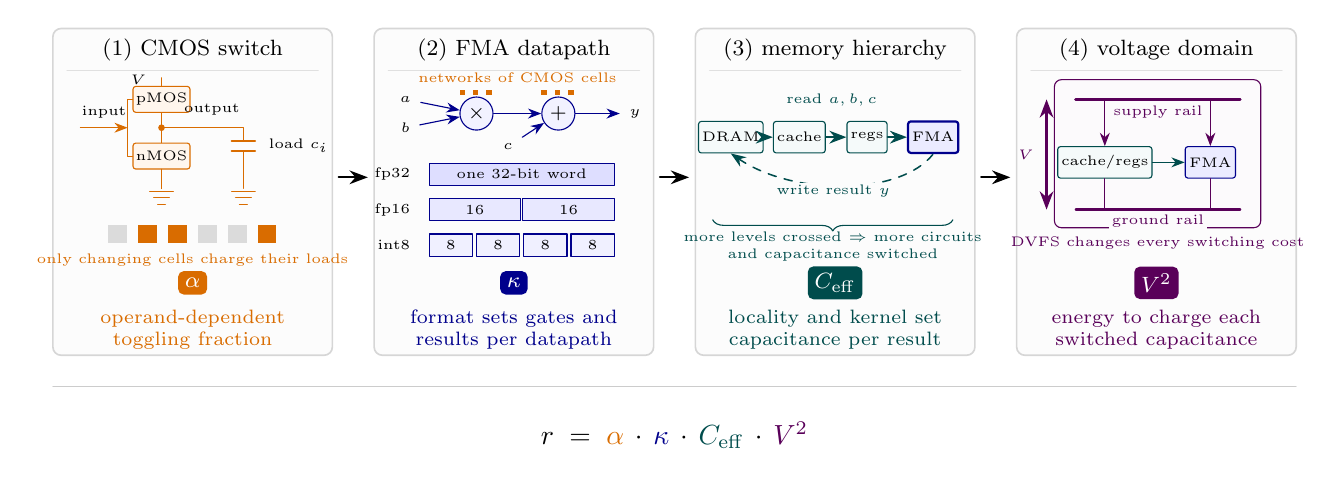
\begin{tikzpicture}[
		>=Stealth, line join=round, line cap=round,
		panel/.style={draw=black!16, fill=black!1, rounded corners=3pt,
			line width=0.6pt},
		badge/.style={rounded corners=2pt, inner sep=2.5pt,
			font=\footnotesize},
		note/.style={font=\scriptsize, align=center},
		title/.style={font=\footnotesize},
		tiny/.style={font=\tiny},
		mos/.style={font=\tiny, draw=colCov, fill=orange!7,
			rounded corners=1pt, minimum width=0.62cm, minimum height=0.33cm,
			inner sep=1pt},
		logic/.style={font=\scriptsize, draw=colTrace, fill=blue!5,
			circle, minimum size=0.42cm, inner sep=0pt},
		fma/.style={font=\tiny, draw=colTrace, fill=blue!8,
			rounded corners=1pt, minimum height=0.4cm, inner sep=1.5pt},
		mem/.style={font=\tiny, draw=colDec, fill=teal!4,
			rounded corners=1pt, minimum height=0.4cm, inner sep=1.3pt}]

		% ============ (1) complementary CMOS switching --- alpha ============
		\begin{scope}[shift={(0,0)}]
			\draw[panel] (0,0.1) rectangle (3.55,4.25);
			\node[title] at (1.775,3.98) {(1) CMOS switch};
			\draw[black!12] (0.18,3.72) -- (3.37,3.72);

			\node[mos] (pmos) at (1.38,3.35) {pMOS};
			\node[mos] (nmos) at (1.38,2.63) {nMOS};
			\draw[colCov, line width=0.65pt]
				(1.38,3.62) -- (pmos)
				(pmos) -- (1.38,2.99) -- (nmos) -- (1.38,2.22);
			\node[tiny, black, anchor=east] at (1.31,3.60) {\(V\)};
			\draw[colCov] (1.23,2.18) -- (1.53,2.18)
				(1.28,2.10) -- (1.48,2.10) (1.33,2.02) -- (1.43,2.02);
			\fill[colCov] (1.38,2.99) circle (1.2pt);
			\draw[->, colCov] (0.35,2.99) -- (0.95,2.99)
				node[tiny, black, midway, above] {input};
			\draw[colCov] (0.95,2.99) -- (0.95,3.35) -- (pmos.west)
				(0.95,2.99) -- (0.95,2.63) -- (nmos.west);
			\draw[colCov] (1.38,2.99) -- (2.42,2.99) -- (2.42,2.82);
			\draw[colCov, line width=0.7pt] (2.27,2.82) -- (2.57,2.82);
			\draw[colCov, line width=0.7pt] (2.27,2.69) -- (2.57,2.69);
			\draw[colCov] (2.42,2.69) -- (2.42,2.22);
			\draw[colCov] (2.27,2.18) -- (2.57,2.18)
				(2.32,2.10) -- (2.52,2.10) (2.37,2.02) -- (2.47,2.02);
			\node[tiny, anchor=west] at (2.62,2.76) {load \(c_i\)};
			\node[tiny, anchor=south] at (2.02,3.02) {output};

			% An operand changes only some of the many cells in a datapath.
			\foreach \x/\c in {0.82/gray!28,1.20/colCov,
				1.58/colCov,1.96/gray!28,2.34/gray!28,2.72/colCov}
				\fill[\c] (\x-0.12,1.52) rectangle (\x+0.12,1.76);
			\node[tiny, text=colCov] at (1.775,1.31)
				{only changing cells charge their loads};
			\node[badge, fill=colCov, text=white] at (1.775,1.02)
				{\(\alpha\)};
			\node[note, text=colCov] at (1.775,0.43)
				{operand-dependent\\toggling fraction};
		\end{scope}

		\draw[->, thick] (3.63,2.36) -- (4.00,2.36);

		% ============ (2) bit-width-selected FMA --- kappa ============
		\begin{scope}[shift={(4.08,0)}]
			\draw[panel] (0,0.1) rectangle (3.55,4.25);
			\node[title] at (1.775,3.98) {(2) FMA datapath};
			\draw[black!12] (0.18,3.72) -- (3.37,3.72);

			\node[tiny] (ain) at (0.40,3.35) {\(a\)};
			\node[tiny] (bin) at (0.40,2.99) {\(b\)};
			\node[logic] (mul) at (1.30,3.17) {\(\times\)};
			\node[logic] (add) at (2.34,3.17) {\(+\)};
			\node[tiny] (cin) at (1.70,2.75) {\(c\)};
			\draw[->, colTrace] (ain) -- (mul);
			\draw[->, colTrace] (bin) -- (mul);
			\draw[->, colTrace] (mul) -- (add);
			\draw[->, colTrace] (cin) -- (add);
			\draw[->, colTrace] (add) -- (3.12,3.17)
				node[tiny, black, right] {\(y\)};
			\foreach \x in {1.12,1.29,1.46,2.16,2.33,2.50}
				\fill[colCov]
					(\x-0.035,3.405) rectangle (\x+0.035,3.475);
			\node[tiny, text=colCov] at (1.82,3.62) {networks of CMOS cells};

			% A fixed-width fabric holds one wide word or several narrow words.
			\node[tiny, anchor=east] at (0.58,2.40) {fp32};
			\draw[colTrace, fill=blue!13] (0.70,2.26) rectangle (3.05,2.54);
			\node[tiny] at (1.875,2.40) {one 32-bit word};
			\node[tiny, anchor=east] at (0.58,1.95) {fp16};
			\foreach \x in {0.70,1.89}
				\draw[colTrace, fill=blue!9] (\x,1.81) rectangle (\x+1.16,2.09);
			\node[tiny] at (1.28,1.95) {16};
			\node[tiny] at (2.47,1.95) {16};
			\node[tiny, anchor=east] at (0.58,1.50) {int8};
			\foreach \x in {0.70,1.30,1.90,2.50}
				\draw[colTrace, fill=blue!6] (\x,1.36) rectangle (\x+0.55,1.64);
			\foreach \x in {0.975,1.575,2.175,2.775}
				\node[tiny] at (\x,1.50) {8};
			\node[badge, fill=colTrace, text=white] at (1.775,1.02)
				{\(\kappa\)};
			\node[note, text=colTrace] at (1.775,0.43)
				{format sets gates and\\results per datapath};
		\end{scope}

		\draw[->, thick] (7.71,2.36) -- (8.08,2.36);

		% ============ (3) memory hierarchy and operand path --- C_eff ============
		\begin{scope}[shift={(8.16,0)}]
			\draw[panel] (0,0.1) rectangle (3.55,4.25);
			\node[title] at (1.775,3.98) {(3) memory hierarchy};
			\draw[black!12] (0.18,3.72) -- (3.37,3.72);
			\node[mem, minimum width=0.55cm] (dram) at (0.45,2.87) {DRAM};
			\node[mem, minimum width=0.58cm] (cache) at (1.32,2.87) {cache};
			\node[mem, minimum width=0.48cm] (reg) at (2.18,2.87) {regs};
			\node[fma, minimum width=0.52cm, line width=0.8pt]
				(memfma) at (3.02,2.87) {FMA};
			\draw[->, colDec, line width=0.7pt] (dram) -- (cache);
			\draw[->, colDec, line width=0.7pt] (cache) -- (reg);
			\draw[->, colDec, line width=0.7pt] (reg) -- (memfma);
			\node[tiny, text=colDec] at (1.73,3.34)
				{read \(a,b,c\)};
			\draw[<-, colDec, dashed, line width=0.55pt]
				(dram.south) .. controls (1.25,2.12) and (2.60,2.12) .. (memfma.south);
			\node[tiny, text=colDec, fill=black!1, inner sep=1pt]
				at (1.75,2.18) {write result \(y\)};
			\draw[decorate, decoration={brace, amplitude=4pt, mirror}, colDec]
				(0.22,1.82) -- (3.27,1.82);
			\node[tiny, text=colDec, align=center] at (1.745,1.48)
				{more levels crossed \(\Rightarrow\) more circuits\\and capacitance switched};
			\node[badge, fill=colDec, text=white] at (1.775,1.02)
				{\(C_{\mathrm{eff}}\)};
			\node[note, text=colDec] at (1.775,0.43)
				{locality and kernel set\\capacitance per result};
		\end{scope}

		\draw[->, thick] (11.79,2.36) -- (12.16,2.36);

		% ============ (4) one supply across that same path --- V^2 ============
		\begin{scope}[shift={(12.24,0)}]
			\draw[panel] (0,0.1) rectangle (3.55,4.25);
			\node[title] at (1.775,3.98) {(4) voltage domain};
			\draw[black!12] (0.18,3.72) -- (3.37,3.72);
			\draw[violet!70!black, fill=violet!2, rounded corners=2.5pt]
				(0.48,1.72) rectangle (3.10,3.60);
			\draw[violet!70!black, line width=1.05pt] (0.75,3.35) -- (2.84,3.35);
			\node[tiny, text=violet!70!black, fill=violet!2, inner sep=1pt,
				anchor=north] at (1.795,3.31) {supply rail};
			\draw[violet!70!black, line width=0.8pt] (0.75,1.95) -- (2.84,1.95);
			\node[tiny, text=violet!70!black, fill=violet!2, inner sep=1pt,
				anchor=north] at (1.795,1.92) {ground rail};
			\node[mem] (diemem) at (1.12,2.55) {cache/regs};
			\node[fma] (diefma) at (2.46,2.55) {FMA};
			\draw[->, colDec] (diemem) -- (diefma);
			\draw[->, violet!70!black] (1.12,3.35) -- (diemem);
			\draw[->, violet!70!black] (2.46,3.35) -- (diefma);
			\draw[violet!70!black] (diemem.south) -- (1.12,1.95);
			\draw[violet!70!black] (diefma.south) -- (2.46,1.95);
			\draw[<->, violet!70!black, line width=0.8pt]
				(0.38,1.95) -- (0.38,3.35);
			\node[tiny, text=violet!70!black, anchor=east] at (0.34,2.65)
				{\(V\)};
			\node[tiny, text=violet!70!black] at (1.79,1.52)
				{DVFS changes every switching cost};
			\node[badge, fill=violet!70!black, text=white] at (1.775,1.02)
				{\(V^2\)};
			\node[note, text=violet!70!black] at (1.775,0.43)
				{energy to charge each\\switched capacitance};
		\end{scope}

		% ============ assembled equation ============
		\draw[black!20] (0,-0.30) -- (15.79,-0.30);
		\node[font=\normalsize] at (7.895,-0.92)
			{\(r \;=\;
			{\color{colCov}\alpha}\,\cdot\,
			{\color{colTrace}\kappa}\,\cdot\,
			{\color{colDec}C_{\mathrm{eff}}}\,\cdot\,
			{\color{violet!70!black}V^2}\)};

	\end{tikzpicture}%
	}
\end{frame}


% ================================================================
% SLIDE 5: Measuring the bands on an A100
% ================================================================
\begin{frame}{How Wide Are the Bands? Measured on an A100}
	\small
	We measured the bands directly on an NVIDIA A100:
	\par\normalsize

	\vspace{1mm}
	\begin{columns}[c,onlytextwidth]
		\begin{column}{0.52\textwidth}
			\centering
			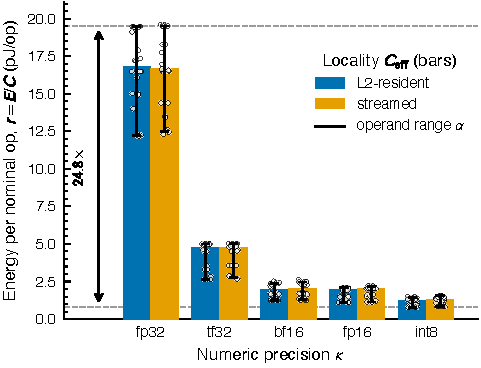
\includegraphics[width=\textwidth]{exchange_band}
		\end{column}
		\begin{column}{0.46\textwidth}
			\small
			\begin{itemize}\itemsep8pt
				\item \textbf{The declared band:} cost per op spans
				{\color{colWarnLine}$\mathbf{24.8\times}$}
				($0.79$--$19.5$\,pJ/op).\\
				{\scriptsize per-factor widths: $\kappa$: $13.5\times$,
				$\alpha$: $1.9\times$, $C_{\mathrm{eff}}$: $1.04\times$,
				$V^2$: ${\approx}1.5\times$ (assumed)}
				\item \textbf{The overhead band:} idle draw wanders over
				$P_0 \in [60,\,101]$\,W --- a $41$\,W band the verifier
				must concede.
			\end{itemize}
		\end{column}
	\end{columns}
\end{frame}


% ================================================================
% SLIDE: results --- how much hides, and what each capability buys back
% ================================================================
\begin{frame}{How Much Compute Can Hide?}
	\begin{columns}[c,onlytextwidth]
		\begin{column}{0.50\textwidth}
			\small
			Define
			$\beta \equiv C_{\mathrm{covert}}^{\mathrm{max}} / C_{\max}$
			\begin{itemize}\itemsep3pt
				\item $\beta = 1.16$ --- just power + a checked precision
				declaration
				\item $\beta =\ ?$ --- clock \& locality: not measurable
				with power alone, nor by our experiments
				\item $\beta = 0.34$ --- re-execute the declared work (a
				hardware gap persists)
				\item $\beta = 0.07$ --- restrict covert work to being
				\emph{useful}
			\end{itemize}

		\end{column}
		\begin{column}{0.48\textwidth}
			\centering
			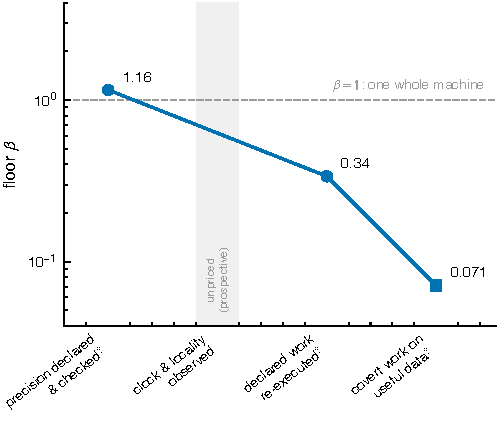
\includegraphics[width=0.88\textwidth]{figures/capability_ladder_talk}\\[1pt]
		\end{column}
	\end{columns}
\end{frame}


% ================================================================
% SLIDE: Limitations
% ================================================================
\begin{frame}{Limitations}
	\small
	\begin{itemize}\itemsep5pt
		\item One vendor, one GPU model, one cluster: the numbers are
		A100-specific (but maths/physics is general).
		\item DVFS never swept (platform denied clock locking)
		\item Energy read from on-die NVML telemetry; in practice an
		off-chip meter adds its own uncertainties
		\item Single device: facility scale is a multi-resource allocation
		problem (shared cooling, work placement, etc.).
		\item Everything is time-integrated;
		richer trace models, multiple channels, or attested telemetry are
		outside it and may do better.
	\end{itemize}
\end{frame}


% ================================================================
% SLIDE 8: Takeaway
% ================================================================
\begin{frame}{Summary}
	\begin{itemize}\itemsep14pt
		\item \textbf{Verification} is important for AI governance.
		\item \textbf{Off-chip analogue measurements} (e.g.\ power) can be
		used for verification.
		\item Power measurements $+$ prover declarations $+$ reasonable
		assumptions constrain covert compute to
		$C_{\mathrm{covert}} \lesssim 7\%$ of machine capacity.
		\item Extending to more realistic, representative \textbf{hardware}
		is the next goal.
	\end{itemize}

	\vfill
	\centering
	{\footnotesize \emph{Can Power Draw Constrain Covert Compute?} ---
	Kimpson, Baker, Graham, Friedman, Rafla, Joseph\\
	\href{mailto:tom.kimpson@unimelb.edu.au}{tom.kimpson@unimelb.edu.au}}
\end{frame}



\end{document}
